\documentclass[emulatestandardclasses]{scrartcl}
\usepackage{graphicx}
\usepackage{color}
\usepackage[ngerman]{babel}
\usepackage{hyperref}
\usepackage{fullpage}
\usepackage[utf8]{inputenc}
\usepackage{calc} 
\usepackage{enumitem}
\usepackage{titlesec}
\newcommand{\todo}[1]{\textcolor{red}{TODO: #1}\PackageWarning{TODO:}{#1!}}
\date{\vspace{-3ex}}
\begin{document}

\title{
	\includegraphics*[width=0.75\textwidth]{ErstesSem/images/hu_logo.png}\\
	\vspace{24pt}
	Pragmatismus}
\subtitle{\vspace{10pt}Lesegruppe WS 17/18\\
          Philosophisches Institut I \\ 
          Humboldt Universit"at zu Berlin}
\author{Lennard Wolf\\
        \small{\href{mailto:lennard.wolf@student.hu-berlin.de}{lennard.wolf@student.hu-berlin.de}}}
\maketitle
\begin{abstract}
Pragmatism was a philosophical tradition that originated in the United States around 1870. The core of pragmatism was the pragmatist maxim, a rule for clarifying the contents of hypotheses by tracing their ‘practical consequences’. In the work of Peirce and James, the most influential application of the pragmatist maxim was to the concept of truth. But the pragmatists have also tended to share a distinctive epistemological outlook, a fallibilist anti-Cartesian approach to the norms that govern inquiry. It was not until the 1970s that interest in the writings of the Pragmatists became widespread and pragmatist ideas were recognized as able to make a major contribution to philosophy. (Source: \url{https://plato.stanford.edu/entries/pragmatism/})

\end{abstract}
\newpage

\tableofcontents
%\listoffigures
\newpage


\section{The Present Dilemma in Philosophy / What Pragmatism Means\\(26.10.17)}

\subsection{The Present Dilemma in Philosophy}

\begin{itemize}
  \item Source: \url{https://brocku.ca/MeadProject/James/James_1907/James_1907_01.html}
  \item Personal philosophy: "`it is our individual way of just seeing and feeling the total push and pressure of the cosmos."'
  \item Philosophy is at once the most sublime and the most trivial of human pursuits. It works in the minutest crannies and it opens out the widest vistas. It 'bakes no bread,' as has been said, but it can inspire our souls with courage; and repugnant as its manners, its doubting and challenging, its quibbling and dialectics, often are to common people, no one of us can get along without the far-flashing beams of light it sends over the world's perspectives. These illuminations at least, and the contrast effects of darkness and mystery that accompany them, give to what it says an interest that is much more than professional. - hach
  \item He trusts his temperament. Wanting a universe that suits it
  \item Modern people are caught between their spiritual needs and scientific standards. Where will these people look for in philosophy?
  \item You want a system that will combine both things, the scientific loyalty to facts and willingness to take account of them, the spirit of adaptation and accommodation, in short, but also the old confidence in human values and the resultant spontaneity, whether of the religious or of the romantic type. And this is. then your dilemma: you find the two parts of your quaesitum5 hopelessly separated. You find empiricism with inhumanism and irreligion; or else you find a rationalistic philosophy that indeed may call itself religious, but that keeps out of all definite touch with concrete facts and joys and sorrows.
  \item The different temperaments are both in some sense right and in some sense right, pragmatism will bring them together
\end{itemize}

\subsection{What Pragmatism Means}

\begin{itemize}
  \item Source: \url{https://brocku.ca/MeadProject/James/James_1907/James_1907_02.html}
  \item The pragmatic method is primarily a method of settling metaphysical disputes that otherwise might be interminable. 
  \item Whenever a dispute is serious, we ought to be able to show some practical difference that must follow from one side or the other's being right.
  \item beliefs are really rules for action, so to develop a thought's meaning, we need only determine what conduct it is fitted to produce [hä? dafür muss ich wissen welches verhalten gut ist. regress?]
  \item It is astonishing to see how many philosophical disputes collapse into insignificance the moment you subject them to this simple test of tracing a concrete consequence.
  \item There is absolutely nothing new in the pragmatic method. 
  \item He turns towards concreteness and adequacy, towards facts, towards action, and towards power.
  \item At the same time it does not stand for any special results. It is a method only.
  \item Its a \emph{theory of truth}
  \item "`\emph{Ideas (which themselves are but parts of our experience) become true just in so far as they help us to get into satisfactory relation with other parts of our experience}"' $\rightarrow$ "`true in so far"'
  \item Man hat set of beliefs, dann werden diese aus irgendeinem Grund nicht mehr valide, dann werden sie angepasst, dann hat man neue Wahrheit (genetic theory)
  \item Wahrheit ist also mehr "`Wahrerheit"'
  \item It must both lean on old truth and grasp new fact; and its success (as I said a moment ago) in doing this, is a matter for the individual's appreciation. When old truth grows, then, by new truth's addition, it is for subjective reasons.
  \item  'to be true' means only to perform this marriage-function (between old truth and new knowledge)
  \item pragmatism may be a happy harmonizer of empiricist ways of thinking, with the more religious demands of human beings.
  \item truth is one species of good
\end{itemize}

\subsubsection{Fragen}

\begin{itemize}
  \item Begründung für Pragmatismus? Er sagt keine Doktrin aber ist actionability nicht eine Doktrin?
  \item Läuft es am ende nicht auf Empirismus raus? Was ist die direkte Unterscheidung zum Empirismus? Wird im Pragmatismus einfach die Atombombe nicht erfunden, weil es actionable ethics gibt?
  \item Wenn ich mich entscheiden soll, ob ich Pragmatismus akzeptiere, und ja sagen bedeutet, dass für mich dadurch einen neuen Holocaust machen wahr wird, und damit meine glorreiche Meisterrasse regieren kann, nein sagen aber bedeutet, dass ich intellektuell da nicht so einfach davon komme, dann müsste ich doch nein sagen?
  \item Pragmatismus setzt sich doch selbst voraus, wenn es die Entscheidung trifft, ob Pragmatismus zu akzeptieren sei doer nicht
  \item Wie kommt Pragmatismus zu Fragestellungen? Wenn Fragestellungen als unnütz abgetan werden, wird auf dem Gebiet auch nicht geforscht, da der Fortschritt nicht nützlich zu sein scheint. Pragmatismus kann doch gar nicht anders, als in einer selbstaffirmativen Ideologie stecken zu bleiben.
  \item Sätze wie " I fully believe in the legitimacy of taking moral holidays" lassen mich zweifeln an der Echtheit des claims, dass Pragmatismus über Empirismus hinausgeht. Und nur statt "Es gibt keinen Gott" zu sagen "Ich weiß nicht ob es einen Gott gibt" erscheint, im Sinne des Pragmatismus, nicht gespickt mit sonderlich vielen Konsequenzen
\end{itemize}

\subsection{Sitzung}

\begin{itemize}
  \item Theorie ist immer eine Praxis und hat Folgen wie auch praktisches Handeln
  \item Was ist Nützlichkeit? 
\end{itemize}

\section{The Will to Believe\\(02.11.17)}

***keine Notizen***

\section{Peirce: On a New List of Categories\\(08.11.17)}

\subsection{Lektürenotizen}

\begin{itemize}
  \item Erstheit ist das Sein von etwas ohne Bezug auf etwas anderes. Es ist das Sein an sich, das als reine Möglichkeit besteht (z. B. Röte als Möglichkeit);
  \item Zweitheit ist die Bestimmung des hier und jetzt von etwas Seiendem (der Gegensatz zweier noch unreflektierter Gefühle); 
  \item Drittheit ist das Prinzip, das hinter den Dingen steht, die mit der Erscheinung verbundene Gesetzmäßigkeit (z. B. dass eine Tür zu öffnen ist, dass ein Tisch eine Ablagefläche hat, der Algorithmus des Computerprogramms).

\end{itemize}



\subsection{Seminar}

\begin{itemize}
  \item Text ist schwer aber grundlegend
  \item manifold of impressions $\rightarrow$ unity
  \item \emph{ground}: Prädikat; Stove is Black
  \item Substance: ganz viele this, it
  \item Being: 
  \item Copula: Verbindungswort, 
  \item Farbe Raum: 
  \item prescience: 
  \item discrimination gebriffe und bedeutung
  \item abstraction: 
  \item prescient 
  \item james und peirce gehen ganz schön aneinander vorbei
  \item 
\end{itemize}



\newpage
%\section{"Uber den Professor}
%Matthias Schlo"sberger ist Heisenbergstipendiat der Deutschen Forschungsgemeinschaft
%an der Humboldt Universit"at zu Berlin mit dem Forschungsprojekt "`Die Erfahrung der Realit"at durch Widerstand"'.
%
%\begin{figure}[h]
%	\centering
%	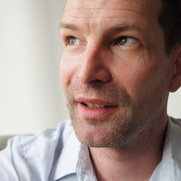
\includegraphics[width=0.3\textwidth]{images/Matthias_Schlossberger.png}
%	\caption{Matthias Schlo"sberger}
%	\label{fig:MS}
%\end{figure}


%\begin{figure}[h]
%	\centering
%	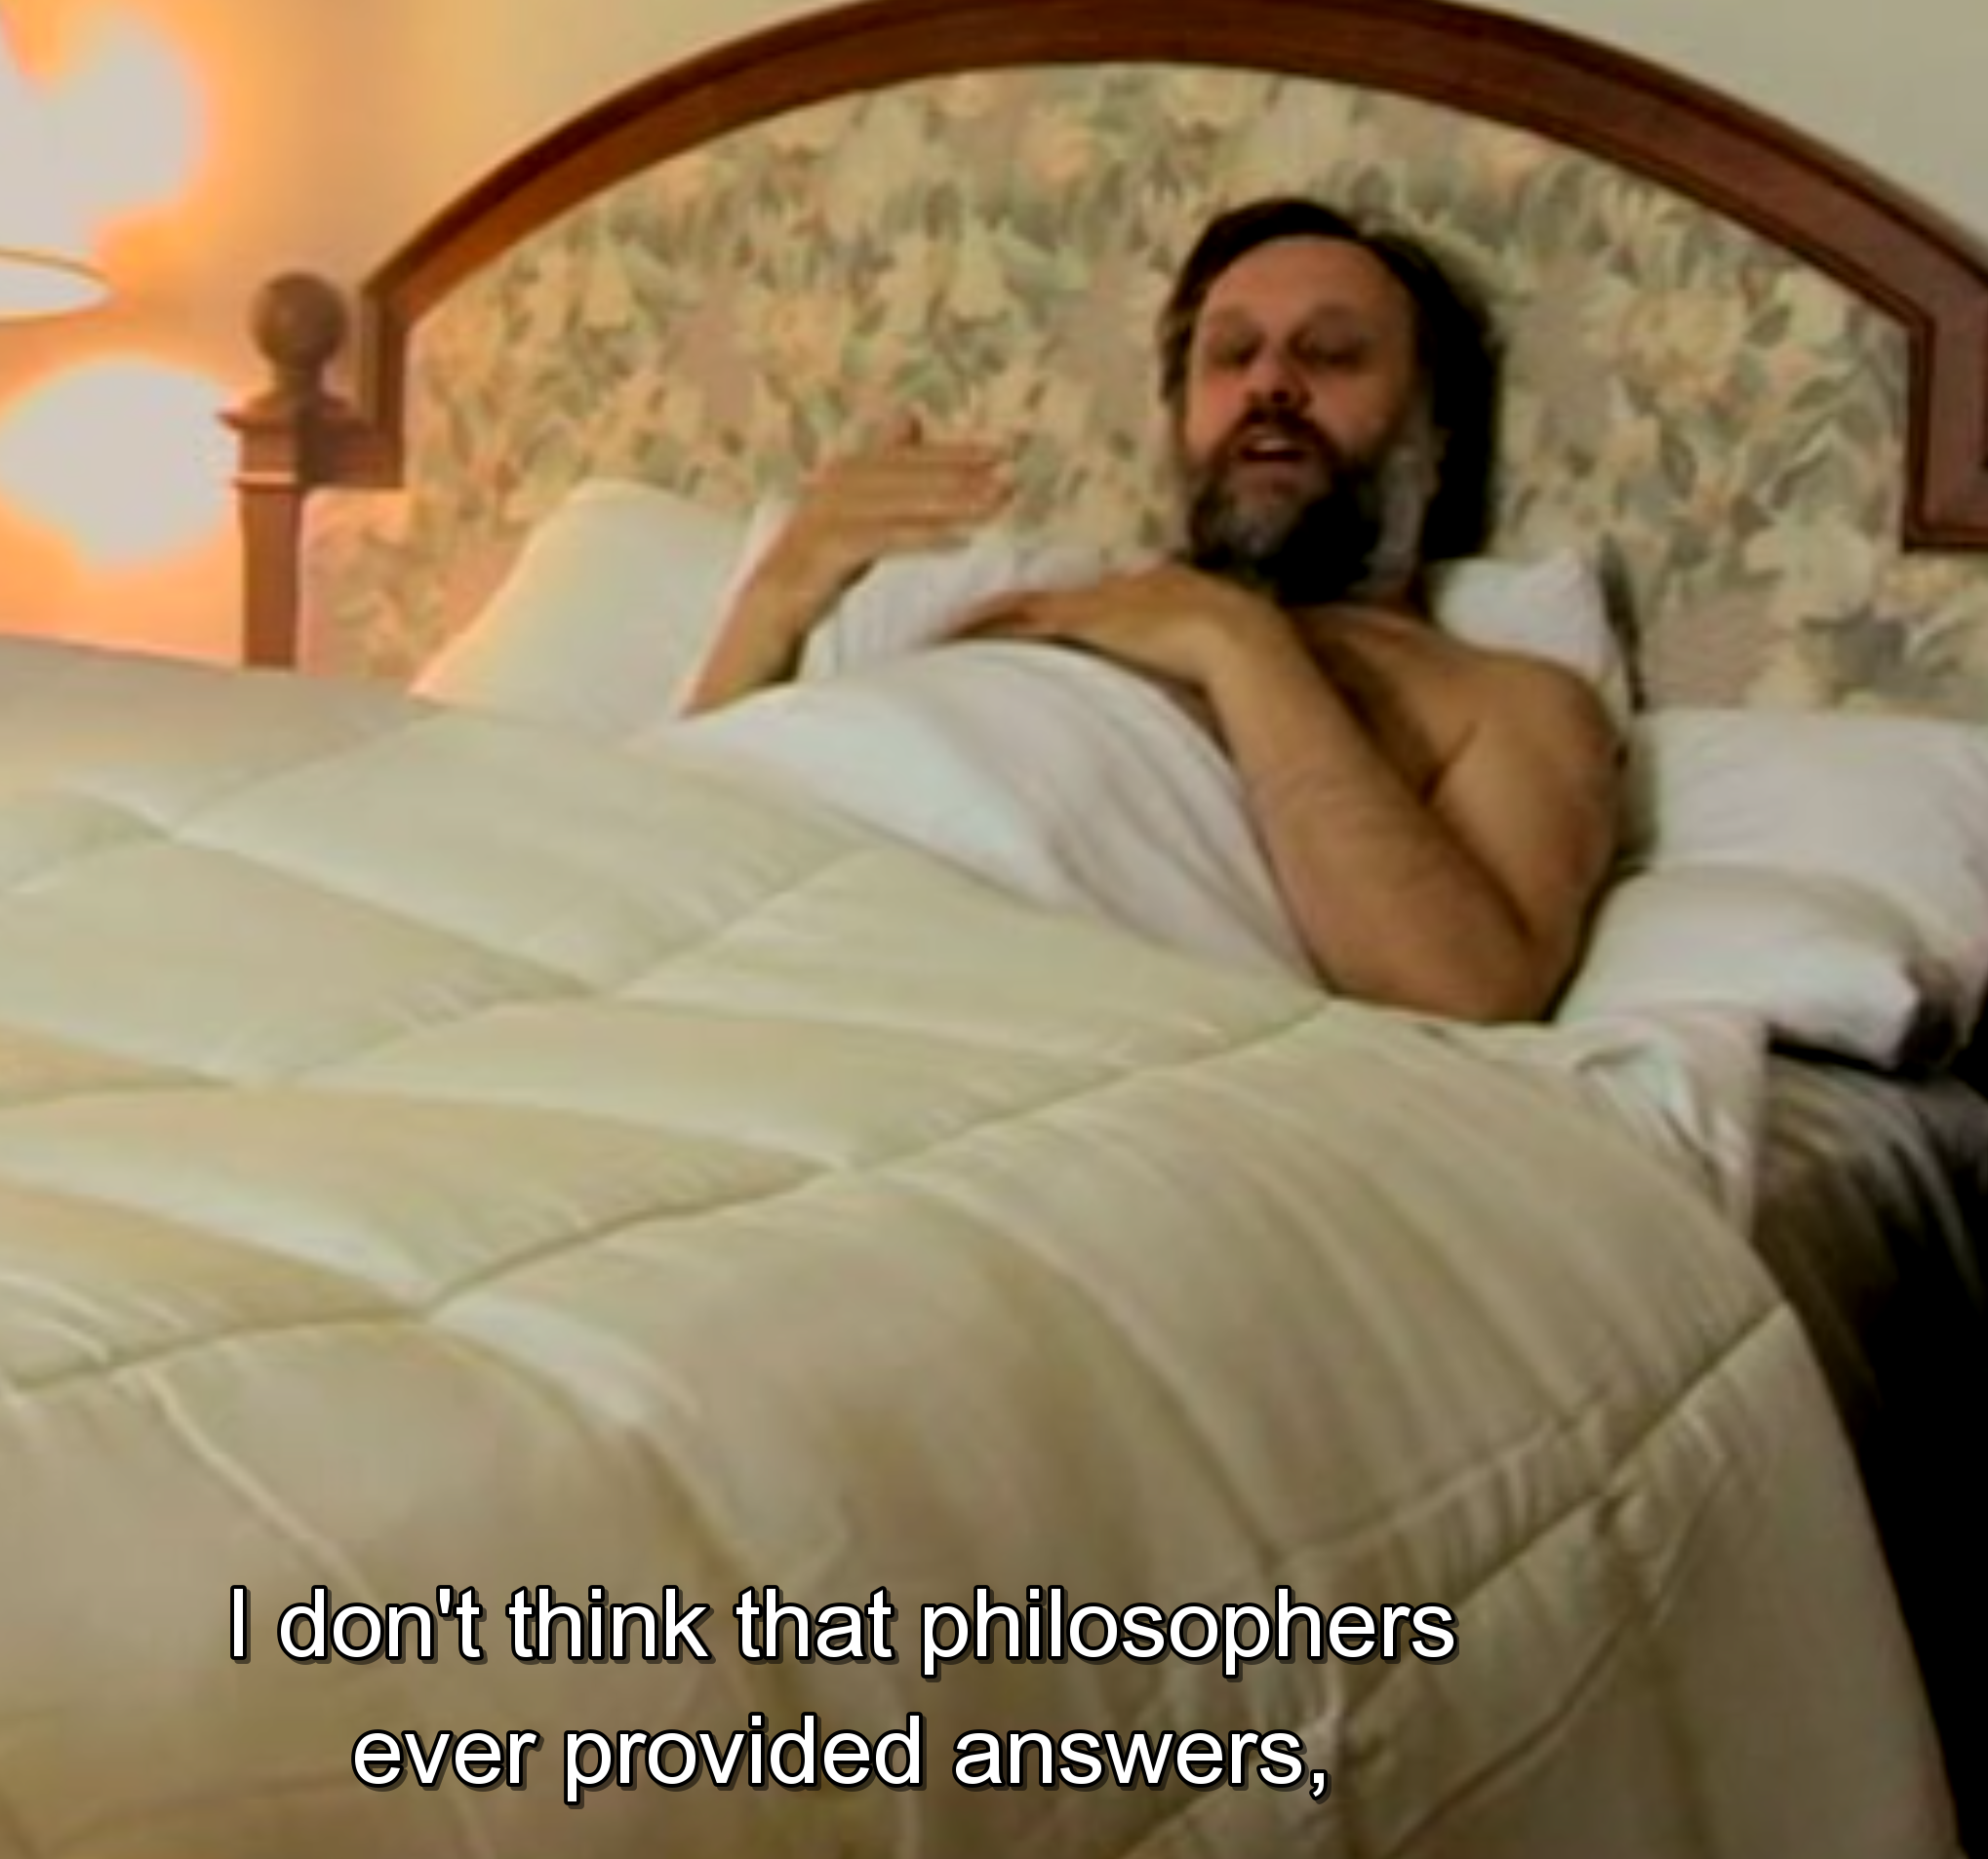
\includegraphics[width=0.5\textwidth]{images/template.png}
%	\caption{Template Bild}
%	\label{fig:template}
%\end{figure}

\end{document}
